\documentclass[12pt]{report}
\usepackage[top=1in,bottom=1in,left=1.5in,right=1.5in]{geometry}
 \usepackage[utf8]{inputenc}
\usepackage[T1]{fontenc}
\usepackage{amsmath,amsthm,amssymb,amsfonts, enumitem, fancyhdr, color, comment, graphicx, environ, stmaryrd,tabu,bbm,titlesec,booktabs,array,lscape,float,longtable}
\usepackage[english]{babel}
\usepackage{hyperref}
\usepackage[ruled,vlined]{algorithm2e}
\usepackage{musicography}
% \usepackage{biblatex}
% \addbibresource{biblio/Dissertation.bib}
\usepackage{helvet}
\usepackage{datetime}
\newdateformat{mydate}{\twodigit{\THEDAY}\ \monthname[\THEMONTH] \THEYEAR}
\renewcommand{\baselinestretch}{1.6}
% \renewcommand{\contentsname}{\center TABLE OF CONTENTS}
\addto\captionsenglish{% Replace "english" with the language you use
    \renewcommand{\contentsname}{TABLE OF CONTENTS}%
    \renewcommand{\listfigurename}{LIST OF FIGURES}
    \renewcommand{\listtablename}{LIST OF TABLES}
}
% \newtheorem{theorem}{Theorem}
% \newtheorem{lemma}{Lemma}
% \newtheorem{proposition}{Proposition}

\titleformat
{\chapter} % command
[display] % shape
{\bfseries\Large} % format
{\centering CHAPTER \thechapter} % label
{0.5ex} % sep
{
    \vspace{1ex}
    \centering
} % before-code
\titlespacing{\chapter}{0cm}{0cm}{1cm}

% The content of the thesis should be in the following order:
%   - Title page
%   - Declaration page
%   - Acknowledgements
%   - Table of Contents
%   - Summary
%   - List of Tables
%   - List of Figures
%   - List of Illustrations
%   - List of Symbols
%   - Main body of thesis
%   - Bibliography
%   - Appendices
 
\begin{document}

% ####################################################################################################
% ####################################################################################################
% Thesis Cover
% ####################################################################################################
% ####################################################################################################

% The thesis cover should contain the following information in BLOCK LETTERS not exceeding 16 points:
%   - Thesis Title
%   - Candidate’s Name
%   - Name of University
%   - Year of first submission

\pagestyle{empty}
\setlength{\parindent}{0cm}
\begin{center}
    {\textbf{\Large Generating new music with deep probabilistic models}}\\
    \vspace{7cm}
    {\textbf{\Large Valentin Vignal}}\\
    \vspace{7cm}
   {\textbf{\Large NATIONAL UNIVERSITY OF SINGAPORE\\}}
    \vspace{1cm}
    {\textbf{\Large 2020}}\\
\end{center}
\newpage


% ####################################################################################################
% ####################################################################################################
% First page with titles
% ####################################################################################################
% ####################################################################################################

% ----- Specification -----
% The title page should contain the following information in BLOCK LETTERS not exceeding 16 points:
%   - Thesis title
%   - Name of Candidate (with qualification(s) in brackets)
%   - The words: “A THESIS SUBMITTED FOR THE DEGREE OF <NAME OF DEGREE>”
%   - Department: DEPARTMENT OF <NAME OF DEPARTMENT>
%   - Name of University: NATIONAL UNIVERSITY OF SINGAPORE
%   - Year of first submission of thesis: If the thesis is resubmitted in a subsequent year, the year of submission to be indicated on the title page should remain as year of first submission.


\pagestyle{empty}
\setlength{\parindent}{0cm}
\begin{center}
    {\textbf{\Large Generating new music with deep probabilistic models}}\\
    \vspace{2cm}
    {\textbf{\Large Valentin Vignal}}\\
    \textbf{(BSc, CentraleSupélec)}\\
    \vspace{2cm}
   {\textbf{\Large A THESIS SUBMITTED FOR THE DEGREE OF MASTER OF COMPUTING\\ DEPARTEMENT OF COMPUTING\\ NATIONAL UNIVERSITY OF SINGAPORE\\}}
    \vspace{2.5cm}
    {\textbf{\Large 2020}}\\
    \vspace{2.5cm}
    {\textbf{\large Advisor:}}\\
    {\textbf{\large Examiners: }}
\end{center}
\newpage

% ####################################################################################################
% ####################################################################################################
% Declaration
% ####################################################################################################
% ####################################################################################################

% ----- Specification -----
% The words on this page should be of a font size of 11 to 12 points. The following should be stated:
% 
% “I hereby declare that this thesis is my original work and it has been written by me in its entirety. I have duly acknowledged all the sources of information which have been used in the thesis.
% This thesis has also not been submitted for any degree in any university previously.”
%
% Candidate should sign at the bottom of the page with the candidate’s name and the date indicated.
% 
%One way for the candidate to insert the scanned page into the thesis (word) document is to save the page as a .jpg file and insert it as a picture into the thesis document before converting the whole document into pdf for submission.

\pagestyle{plain}
\pagenumbering{roman}
\setcounter{page}{2}
\begin{center}
    \textbf{\Large DECLARATION}\\
    \vspace{2cm}
    I hereby declare that this thesis is my original work and it has been written by me in its entirety. I have duly acknowledged all the sources of information which have been used in the thesis.\\
    This thesis has also not been submitted for any degree in any university previously.\\
    \vspace{5cm}
    \begin{figure}[H]
        \centering
        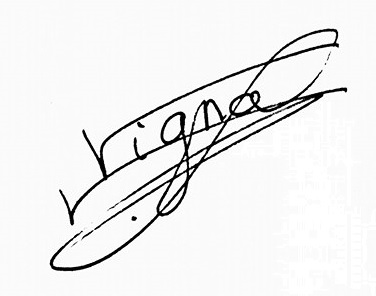
\includegraphics[scale=0.5]{images/Signature2.jpg}
    \end{figure}
    \begin{tabular}{c}
 \hrulefill \\
 Valentin Vignal \\
 \mydate\today\\
\end{tabular}
\end{center}
\newpage

% ####################################################################################################
% ####################################################################################################
% Acknowledgements
% ####################################################################################################
% ####################################################################################################

\begin{center}
    \textbf{\Large ACKNOWLEDGEMENTS}\\
\end{center}

I would like to express my thanks my special thanks or gratitude to my advisor Harold Soh who gave me the opportunity to work on this project combining Artificial Intelligence and Music.

Secondly I would also like to thanks all the member of the research team, and especially the PhD. students Abdul Fatir and Yaqi Xie who, despite their busy schedules, taught me, and help me in many scenarios.

I also yould like to thanks the Doctor Dorien Herremans who gave me some precious advices at the beginning of my project.

\newpage
\tableofcontents
\newpage

% ####################################################################################################
% ####################################################################################################
% Summary
% ####################################################################################################
% ####################################################################################################

\setlength{\parindent}{0.6cm}

% ----- Specification -----
% The thesis must contain a summary of not more than 500 words written in the English Language. If prior approval from the Faculty has been obtained at the time of admission for a thesis to be written in a language other than English, it must contain a summary of not more than 500 words written in that language in addition to a summary not exceeding 500 words written in the English Language. The summary must be included in the thesis.

\begin{center}
    \textbf{\Large SUMMARY}
\end{center}
My asbtract text

% ####################################################################################################
% ####################################################################################################
% List of Tables
% ####################################################################################################
% ####################################################################################################

\listoftables

% ####################################################################################################
% ####################################################################################################
% List of Figures
% ####################################################################################################
% ####################################################################################################

\listoffigures

% ####################################################################################################
% ####################################################################################################
% List of Illustration
% ####################################################################################################
% ####################################################################################################


% ####################################################################################################
% ####################################################################################################
% List of Syhmbols
% #####################################################################################################
% #####################################################################################################
\newpage
\begin{center}
    \textbf{\Large LIST OF SYMBOLS}\\
    \vspace{2cm}
    \begin{table} [ht]
        \begin{center}
            \begin{tabular} {ll}
            AE & Auto Encoder \\
            AI & Artificial Intelligence \\
            CNN & Convolutional Neural Network \\
            GAN & Generative Adversial Network \\
            GRU & Gated Recurrent Unit \\
            KLD & Kullback-Leibler Divergence \\
            LSTM & Long Short-Term Memory \\
            MIDI & Musical Instrument Digital Interface \\
            ML & Machine Learning \\
            MVAE & Multimodal Variational AutoEncoder \\
            NN & Neural Network \\
            RBM & Restricted Bolzmann Machine \\
            ReLU & Rectified Linear Unit \\
            RL & Reinforcement Learning \\
            RMVAE & Recurrent Multimodal Variational AutoEncoder \\
            RNN & Recurrent Neural Network \\
            SGD & Stochastic Gradient Descent \\
            VAE & Variational AutoEncoder \\
            VRAE & Variational Recurrent AutoEncoder \\
            \end{tabular}
        \end{center}
    \end{table}
    
\end{center}
\newpage

\pagenumbering{arabic}

% ####################################################################################################
% ####################################################################################################
% Main body of the thesis
% #####################################################################################################
% #####################################################################################################


% ----------------------------------------------------------------------------------------------------
% Introduction
% ----------------------------------------------------------------------------------------------------
\chapter{Introduction}
My Introduction

% ----------------------------------------------------------------------------------------------------
% Background
% ----------------------------------------------------------------------------------------------------
\chapter{Background}

In this chapter, I will introduce some background knowledge that might be useful to the reader. Since this project is about music generation, I will explain and illustrate some basic concepts about music.

I will consider the Western music using equal temperament and don't consider the inharmonicity of stringed instruments. These are common assumptions in all the existing works about music generation.

% -------------------- Music Representation --------------------

\section{Music representation}

In this section I will explain how musicians represent the music on paper, and from it, how it is possible to represent the music in a abstract way in a computer without encoding any waveforms or actual \textit{sounds}.

\subsection{Musical stave}

It is very useful for anyone to be able to write down their work to save it or share it with someone else. Musicians faced this issue too. They came up with the musical stave :

\begin{figure}[H]
    \centering
    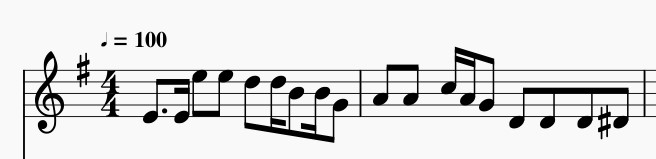
\includegraphics[scale=0.75]{images/music/stave/musical_stave_example.jpg}
    \caption{Musical Stave example}
    \label{fig:musical_stave_example}
\end{figure}

The vertical axis is the frequence axis an the horizontal axis corresponds to the time axis.
In the figure \ref{fig:musical_stave_example}, we know that the tempo is $100 BPM$, that the scale is \textit{G major} and the measure are divided in 4 beats ($4/4$ inscription).
As said previously, the vertical position of a note indicates its frequency :

\begin{figure}[H]
   \begin{minipage}{0.5\textwidth}
     \centering
     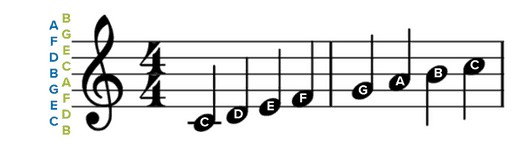
\includegraphics[width=.9\linewidth]{images/music/stave/note_names.jpg}
     \caption{Notes on a musical stave}
     \label{fig:note_names}
   \end{minipage}\hfill
   \begin{minipage}{0.5\textwidth}
     \centering
     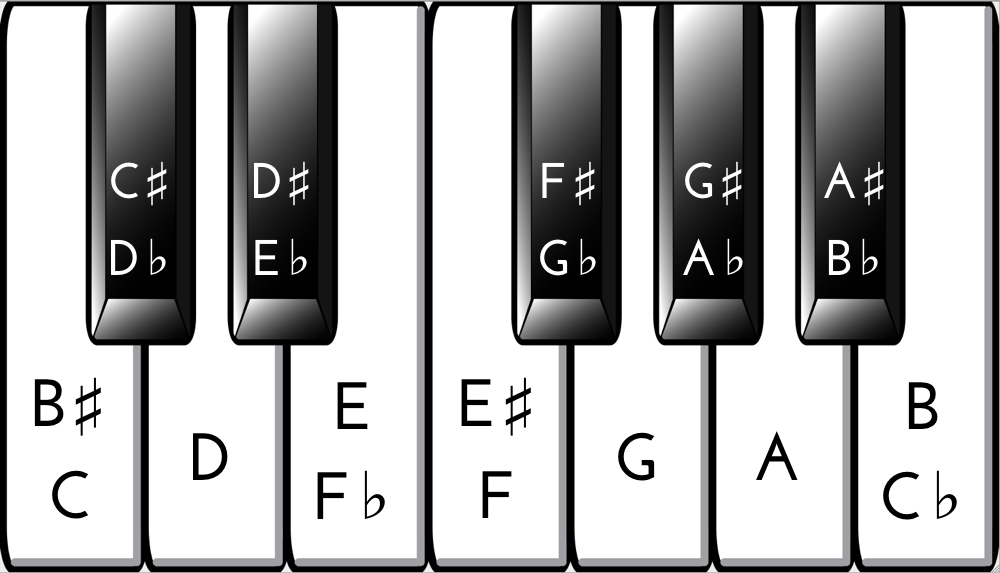
\includegraphics[width=.9\linewidth]{images/music/piano/piano_keys.png}
     \caption{Notes on Piano}
     \label{fig:piano_keys}
   \end{minipage}
\end{figure}

The figures \ref{fig:note_names} and \ref{fig:piano_keys} show the correspondence between the notes on a musical stave and on a piano keyboard. By default the notes correspond to the white keys of the piano (it is the C major scale).

One thing to know is that, between 2 followings notes (or piano keys, including white and black keys), the ratio between the fundamental frequencies of the 2 notes is always equal to $\sqrt{12}$. It means that if we consider the notes $A4$ and $A5$ (2 A in the octaves 4 and 5), the ratio between the fundamental frequencies is $2$. This information will help to understand chords construction.

The length of a note is defined by its shape as shown in the Table \ref{tab:notes_duration}. This table is describing the relation between the length of a note, and its shape on the muscial stave.

\begin{table} [ht]
    \begin{center}
        \begin{tabular} {c|c|c}
            Name & Duration & Symbol \\
            \hline
            Whole note & $4$ beats & {\Large \musWhole} \\ 
            Half note & $2$ beats & {\Large \musHalf} \\
            Quarter note & $1$ beat & {\Large \musQuarter} \\
            Eighth note & $1/2$ beat & {\Large \musEighth} \\
            Sixteenth note & $1/4$ beat & {\Large \musSixteenth} \\
        \end{tabular}
        \caption{Note names and duration}
        \label{tab:notes_duration}
    \end{center}
\end{table}

In this work, we won't consider shorter notes than Sixteenth notes because most of the songs are not using them.


\subsection{MIDI}
\label{seq:midi}

% The \textit{MIDI} format ($.mid$) is a format to save music as a file. However, it doesn't save the actual \textit{sound} of it. The way it works is very similar to the representation of a musical stave.

% In a midi file is a set of instructions. It will save for each instruments, for each notes (pitch) the times when the note starts and ends and some other information (like the velocity et caetera).

% To read a midi file, the computer has a collection of sound for every instruments, notes, velocity et caetera, and plays these sounds depending of the instructions read in the file.

\textit{MIDI} format ($.mid$) is a technical standard that describes a protocol.
It was first used to carry musical messages between electronic instruments, software and devices. These messages are events about note information (for example, pitch, velocity, panning...) an some other parameters (for example, vibrato, volume...). 
The to most important messages are:
\begin{itemize}
    \item \textit{Note on} is indicating that a note has to be played. It contains the channel information (which can be considered as an instrument), the pitch information (what note should be played) and the velocity. We could right an event as follow :
    \begin{equation}
        <NoteOn, 0, 50, 127>
    \end{equation}
    To describe the event \textit{Start to play the note $D3$ with the maximum velocity (127) for the channel (instrument) 0}
    \item \textit{note off} is indicating to stop playing a note (like release the keyboard key). The given parameters should be the same as the ones given to the \textit{Note On} event.
    \begin{equation}
        <NoteOff, 0, 50, 127>
    \end{equation}
    will stop the note started with the previous \textit{Note On} event.
\end{itemize}

Each note is associated with a time value which can be expressed in number of ticks (time division). The header of file should specify how may ticks there are per quarter note.

\subsection{Pianoroll}

The pianoroll is a common representation of a musical stale in the softwares for music production.

\begin{figure}[H]
    \centering
    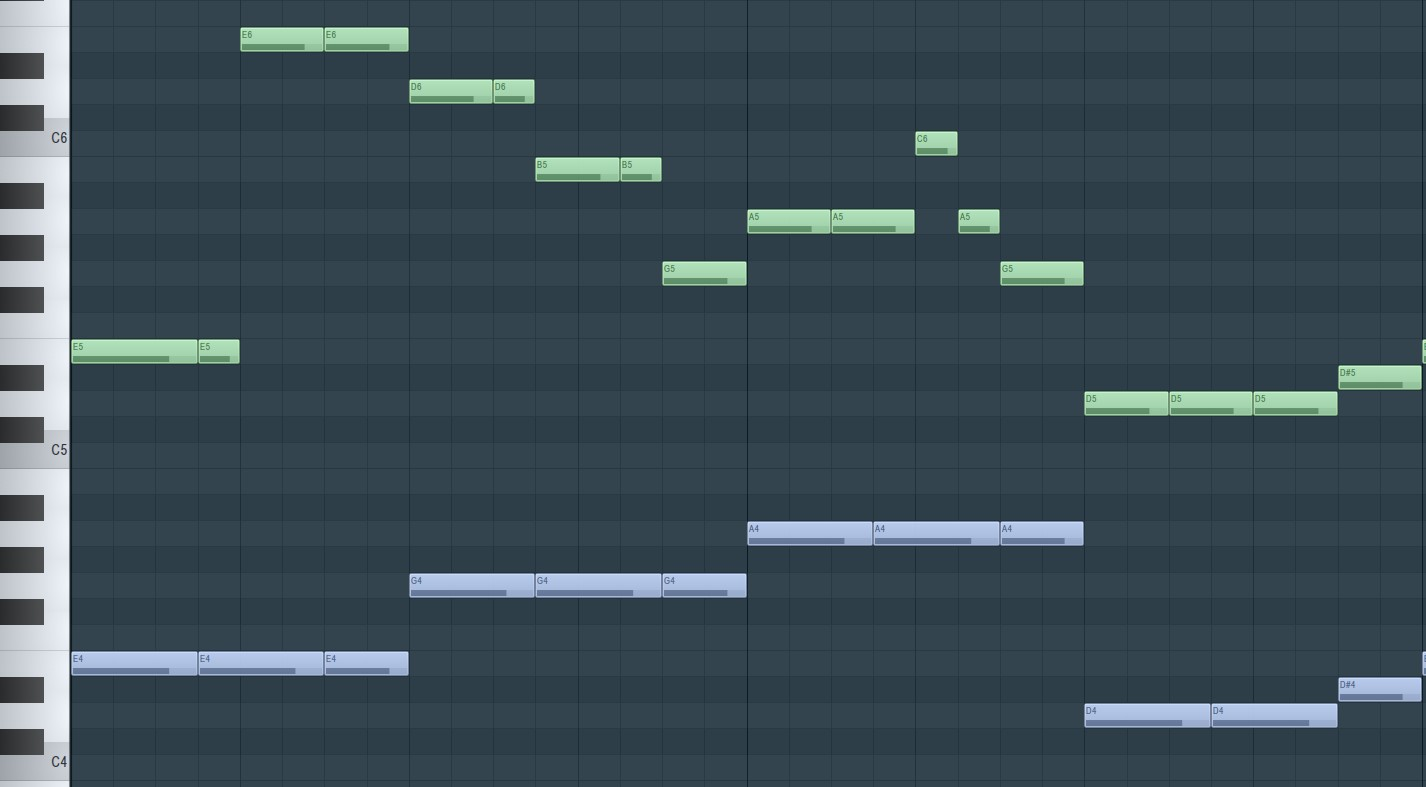
\includegraphics[width=0.75 \textwidth]{images/music/pianoroll/pianoroll_flstudio.jpg}
    \caption{Pianoroll example from the software FL Studio}
    \label{fig:pianoroll_flstudio}
\end{figure}

The figure \ref{fig:pianoroll_flstudio} shows a view of the pianoroll in the famous software \textit{FL Studio}. The composers of electronic music like EDM, Techno et caetera use this view to compose and arrange their songs.

% -------------------- Music Theory --------------------

\section{Music theory}

In this section, I will describe and explain some rules from the music theory which are related to this work. The rules I am going to talk about are the more common ones and most of the songs are following them.

\subsection{Scale and Rhythm}

\subsection*{Scale}

A \textit{scale} is a set of notes. Because the human ear is now used to it, the notes of a scale will sound nice when they are played together. In traditional Western music, it generally consists of 7 notes. They are several types of scales, the most common is the \textit{Major scale} or the \textit{Natural Minor Scale}. For example, the C Major scale uses all the white keys of the piano (Figure \ref{fig:piano_keys}: A, B, C, D, E, F and G), as well as the A Natural Minor scale.

Another type of scales often used by the musicians to creates their \textit{solos} are the \textit{Pentatonic} scales.


\begin{figure}[H]
    \centering
    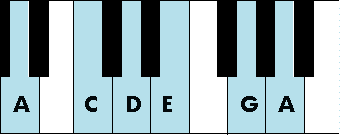
\includegraphics[width=0.5 \textwidth]{images/music/piano/pentatonic_scale.png}
    \caption{C Major Pentatonic scale (or A Minor Pentatonic scale)}
    \label{fig:pentatonic_scale_piano}
\end{figure}

As seen in the Figure \ref{fig:pentatonic_scale_piano}, the C Major pentatonic scale (which uses the same notes as the A Minor pentatonic scale) uses only five notes (A, C, D, E and G) which are contained in the C Major Scale. It is known that playing in this scale will easily produce enjoyable and in tune melodies or any musical parts. 


\subsection{Rhythm}

The rhythm is an important part of the current music like \textit{Pop Music}. It has the tendency to remains consistent through the song and repeat some patterns. It helps the listener to easily follow the progression and allows him to listen what he's expecting.

However, there are no such rules for rhythm as there are for scales and harmonies. This is why classical music is not considered as a rhythmic music.

I this work, I considered and will consider only binary rhythm (each beat is divided into 2 smaller equal beats) and not ternary rhythm (each beat is divided into 3 smaller equal beats) because the binary rhythm is the most common rhythm.

\subsection{Harmonics}

In this section, I will introduce some physical concept about musical sounds and then illustrate how it can explain some musical rules.

\subsubsection{Harmonics}

A sound is a sum of harmonics:

\begin{equation}
    s(t) = \sum_{n=1}^{\infty} \alpha_{n} \sin(n f t + \phi_{n})
\end{equation}
With $f$ the fundamental frequency and $\phi$ the phase difference value.

Let's take an example with the $A4$ note which has a its fundamental frequency equals to $440 Hz$ for a common tuning.
Then the $2^{nd}$ harmonic is $A5$ $880Hz$. So, when an instrument plays a $A4$, all the harmonics of a $A5$ are also present.
Let's take one step further, the $3^{rd}$ harmonic of $A4$ is $E5$ $1320Hz$. It means it is possible to hear a $E5$ from a played $A4$.
The table \ref{tab:A4_harmonics} is referencing the firsts harmonics of the note $A4$.

\begin{table} [ht]
    \begin{center}
        \begin{tabular} {c||c|c|c}
            Harmonic number & Frequency ($Hz$) & Note Name & Musical Interval \\
            \hline
            $1$ & $440$ & $A4$ & Unison \\
            $2$ & $880$ & $A5$ & Octave \\
            $3$ & $1320$ & $E5$ & Fifth \\
            $4$ & $1760$ & $A6$ & Octave \\
            $5$ & $2200$ & $C\sh6$ & Major Third \\
            $6$ & $2640$ & $E6$ & Fifth \\
        \end{tabular}
        \caption{Harmonics of $A4$}
        \label{tab:A4_harmonics}
    \end{center}
\end{table}
From the table \ref{tab:A4_harmonics}, we can notice:
\begin{itemize}
    \item The $A$ and $E$ notes are linked together (\textit{Fifth} or reversed \textit{Fourth} interval).
    \item The $A$ and $C\sh$ notes are linked together (\textit{Major Third} interval).
\end{itemize}


\subsubsection{Chords}

And this is why a Major chord sound nice to the ears. A $A$ $Major$ chord is composed with 3 notes : $A$, $C\sh$ and $E$. All the notes are already contained in the harmonics of a $A$ sound.

A Minor chords ($A$ $Minor$ is $A$, $C$, $E$) will also sounds acceptable to the human ears because $A$ and $C$ share $E$ in their harmonics (\textit{Fifth} interval and \textit{Third Major} interval respectively) 

\subsubsection{Dissonance}

When 2 frequencies are close to each other and added up, it is possible to observe a resonance phenomena:

\begin{figure}[H]
    \centering
    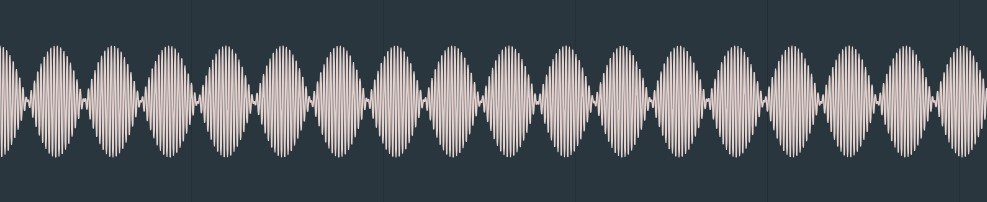
\includegraphics[width=\textwidth]{images/music/waveform/resonance.jpg}
    \caption{Resonance waveform}
    \label{fig:resonance}
\end{figure}
The figure \ref{fig:resonance} shows the waveform generated by a $B4$ ($494Hz$) and a $C5$ ($523Hz$) (\textit{semitone} interval).
This phenomena is explained by the equation:

\begin{equation}
    \cos(f) + \cos(f + \delta f) = 2 \cos(\frac{2f + \delta f}{2}) \cos(\frac{\delta f}{2})
\end{equation}

This phenomena is unpleasant to hear and this is why, musician usually try to avoid to play notes generating a resonance between their harmonics:
\begin{itemize}
    \item \textit{Semitone} interval (ex: $A$ and $A\sh$)
    \item \textit{Tone} interval (ex: $A$ and $B$)
    \item \textit{Tritone} interval (ex: $A$ and $D\sh$)
\end{itemize}


\subsubsection{Harmony}

Either for classical music (Bach Chorales) or pop music (Back Singers), a common method to \textit{fill a song} is to add harmony parts to the lead melody. The harmony parts usually follow the lead melody but on other notes.
An example is provided in the figure \ref{fig:harmony_example}.

\begin{figure}[H]
    \centering
    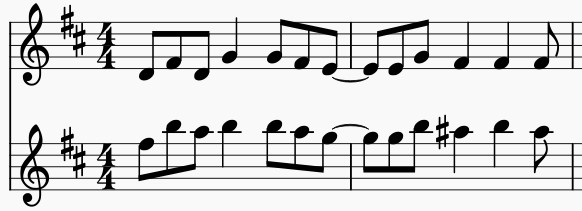
\includegraphics[width=0.75 \textwidth]{images/music/stave/harmony.jpg}
    \caption{Lead voice and its harmony part}
    \label{fig:harmony_example}
\end{figure}

The harmony parts will usually avoid unpleasant interval and mostly try to create the following ones: 
\begin{itemize}
    \item \textit{Octave} and \textit{unison} interval
    \item \textit{Fifth} interval
    \item \textit{Fourth} interval
    \item \textit{Major Third} interval
    \item \textit{Minor Third} interval
\end{itemize}


% -------------------- Music arrangement  --------------------

\section{Music arrangement}

Arranging a song is using all the previous observations and rules to create the harmony parts of a song given the lead melody. It 


% -------------------- Neural Network architecture --------------------

\section{Neural Network architectures}

\subsection{Convolutional neural network}

The convolutional networks are often used on images because they can preserve the spatial information.
A CNN can include two types of layers :
\begin{itemize}
    \item A convolutional layer
    \item A pooling layer
\end{itemize}

\subsubsection{Convolutional Layer}

For a 2D convolution, the convolutional layer which takes as input a tensor of shape \texttt{(height, width, channels)}.
The \textit{filter} of the convolutional layer will have a shape \texttt{(h, w, channels)}.
Then the layer will do a convolutional operation between the filter and the input through the axes corresponding to the \texttt{height} and the \texttt{width}.

\begin{equation}
    y_{\tau} = \sum_{t=0}^{l-1} w_{t} \times x_{\tau + t}
    \label{eq:convo}
\end{equation}

The equation \ref{eq:convo} shows the mathematical transformation for a 1D convolution with $x$ as the input, $w$ as the filter/kernel and $y$ as the output.

\subsubsection{Pooling Layer}

A pooling layer is used to reduce the size of a tensor. It extracts a value from a region of the tensor. It can be:
\begin{itemize}
    \item \textit{Average pooling} takes the average of the region
    \item \textit{Max pooling} takes the maximum of the region
\end{itemize}
The figure \ref{fig:max_pooling} shows how the max pooling operation works.

\begin{figure}[H]
    \centering
    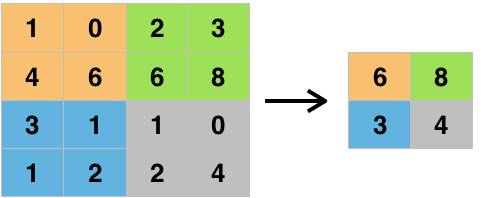
\includegraphics[width=0.75 \textwidth]{images/nn/layers/max_pooling.png}
    \caption{Max pooling operation}
    \label{fig:max_pooling}
\end{figure}

\subsection{AutoEncoder}

An AE is composed of a \textit{encoder} and a \textit{decoder}.
First, the input goes into the encoder. The output of the encoder is the latent space (the hidden layers), which is smaller than the input.
The output of the encoder becomes the input of the decoder. The goal of the decoder is to reconstruct the input from the latent space.
The hidden layers of the AE are smaller than the input which is supposed to force the network to compress the input and reduce its dimensions.
The AE is then forced to learn "high level features" about the inputs.
The figure \ref{fig:autoencoder} illustrates this architecture.

\begin{figure}[H]
    \centering
    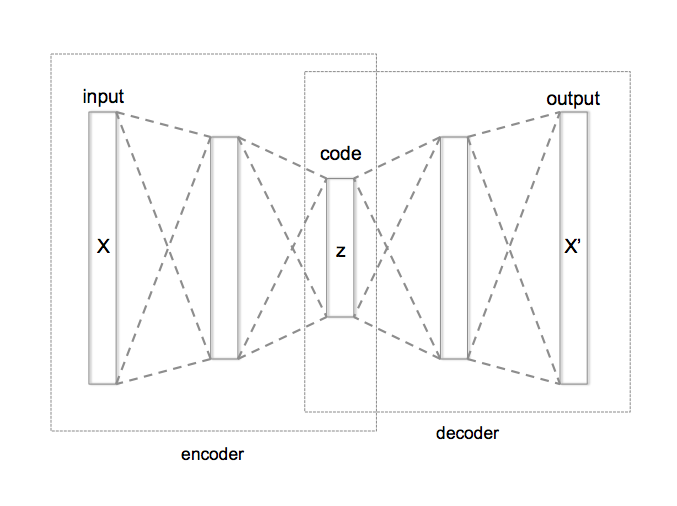
\includegraphics[width=0.75 \textwidth]{images/nn/architectures/autoencoder.png}
    \caption{AutoEncoder}
    \label{fig:autoencoder}
\end{figure}

\subsection{Variational AutoEncoder}
% Multimodal explained in my work part

A VAE is an autoencoder. The steps are the following:
\begin{enumerate}
    \item The input goes first in the encoder which encodes it as a gaussian distribution over the latent space.
    \item A point is sample from this distribution.
    \item This point is decoder by the decoder to reconstruct the input.
\end{enumerate}

By encoding the normal distribution and not directly the latent space, it is possible to regularize the output of the encoder to avoid overfitting and ensure that the latent space as good properties that enable generative process.

To regularize the output of the decoder, an extra term is added to the loss function : Kulback-Leibler Divergence (KLD) between the encoded distribution and the centred and reduced normal distribution :

\begin{equation}
    \mathbb{D}_{KL} (\mathcal{N}(\mu_{encoded}, \sigma_{encoded}), \mathcal{N}(0, 1))
\end{equation}

\subsection{Generative Adversial Network}

GAN are composed of two models that are trained simultaneously:
\begin{itemize}
    \item The \textit{Generator} will learn how to create images that look real
    \item The \textit{Discriminator} will learn how to differentiate real and generated images.
\end{itemize}

The discriminator can be trained with real images and images generated by the generator. The goal of the discriminator is to classify the real images as \textit{"Real"} and the generated images as \textit{"Fake"}.
On the other side, the generator takes some noise as an input to generate an image. And his goal is to make the discriminator classify his generated images as \textit{"Real"}.

\subsection{Recurrent Neural Networks}

A RNN is a neural network where connections between nodes form a direct graph along a temporal sequence. The general architecture is showed in the figure \ref{fig:rnn}.

\begin{figure}[H]
    \centering
    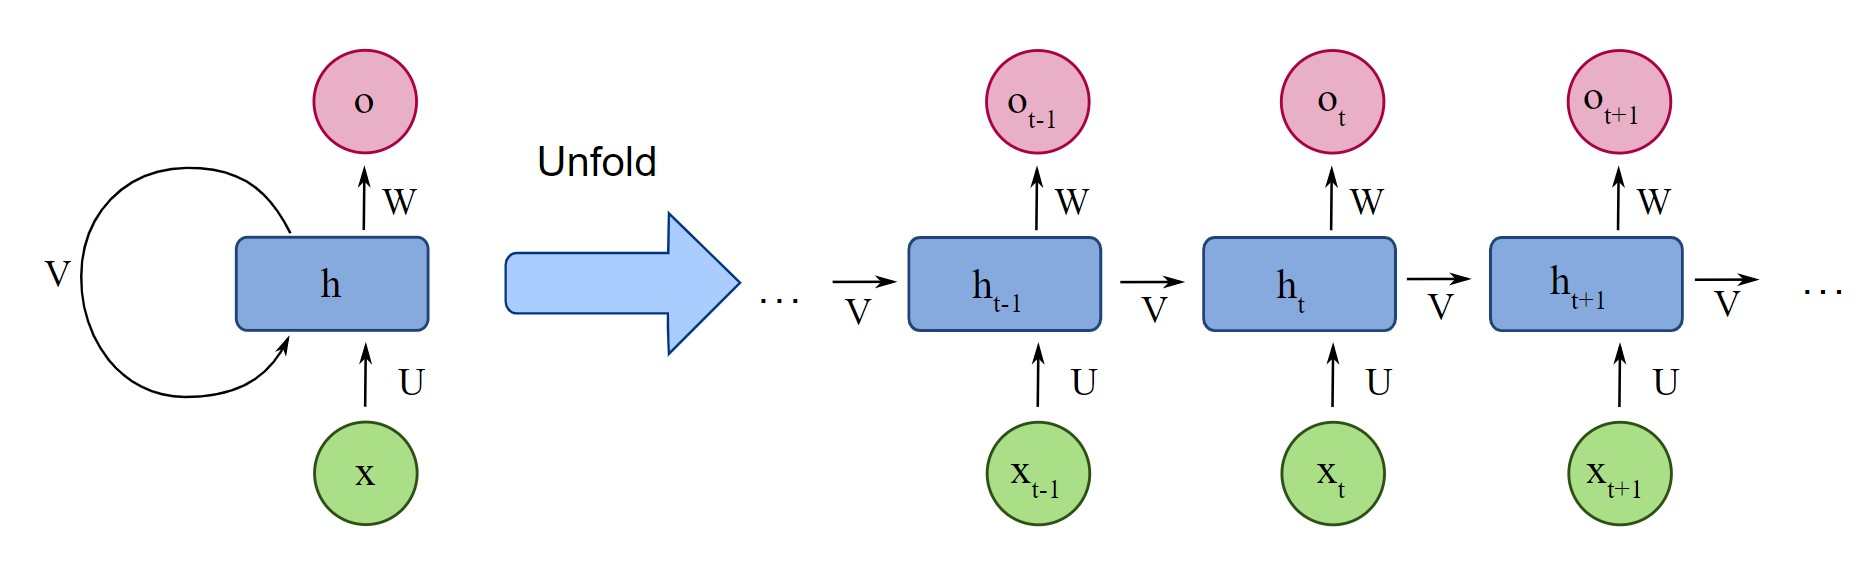
\includegraphics[width=0.75 \textwidth]{images/nn/architectures/rnn.jpg}
    \caption{Recurrent Neural Network}
    \label{fig:rnn}
\end{figure}

The most used cells used are the LSTM cell and the GRU cell. The architectures are showed in the figures \ref{fig:lstm} and \ref{fig:gru}.

\begin{figure}[H]
   \begin{minipage}{0.5\textwidth}
     \centering
     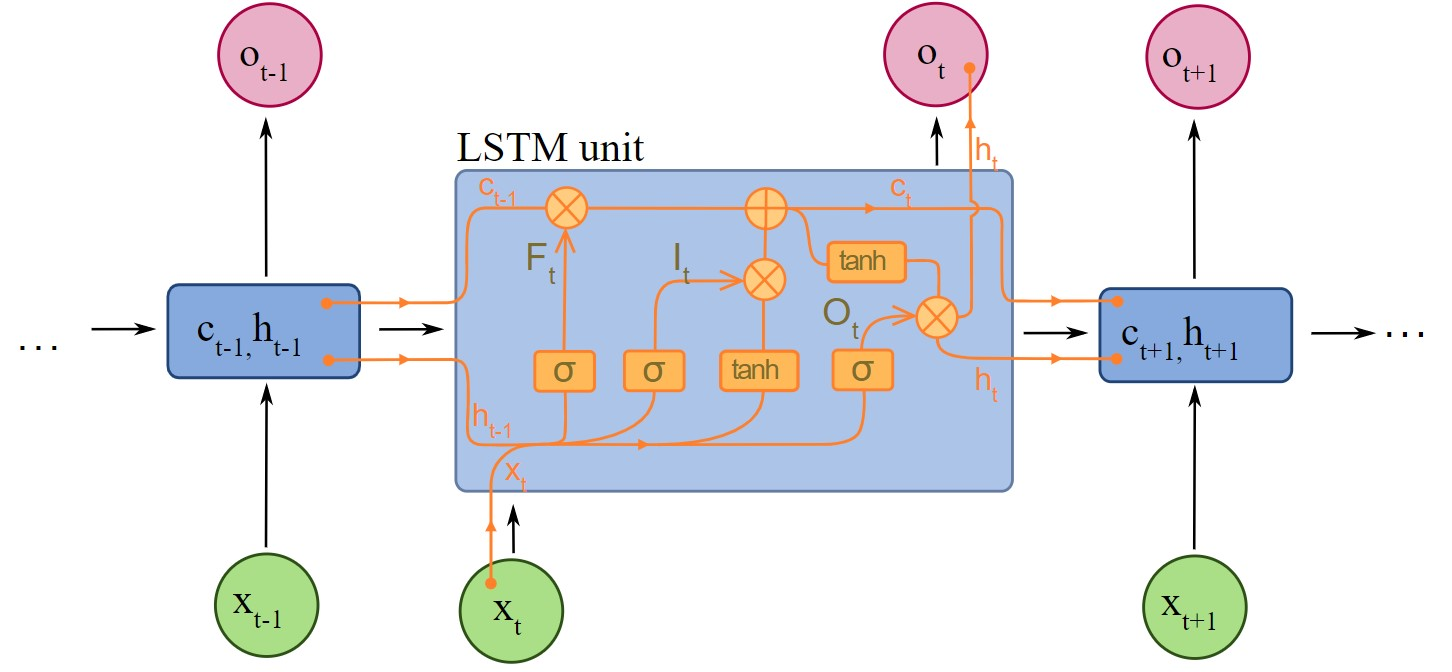
\includegraphics[width=.95\linewidth]{images/nn/layers/lstm.jpg}
     \caption{LSTM cell}
     \label{fig:lstm}
   \end{minipage}\hfill
   \begin{minipage}{0.5\textwidth}
     \centering
     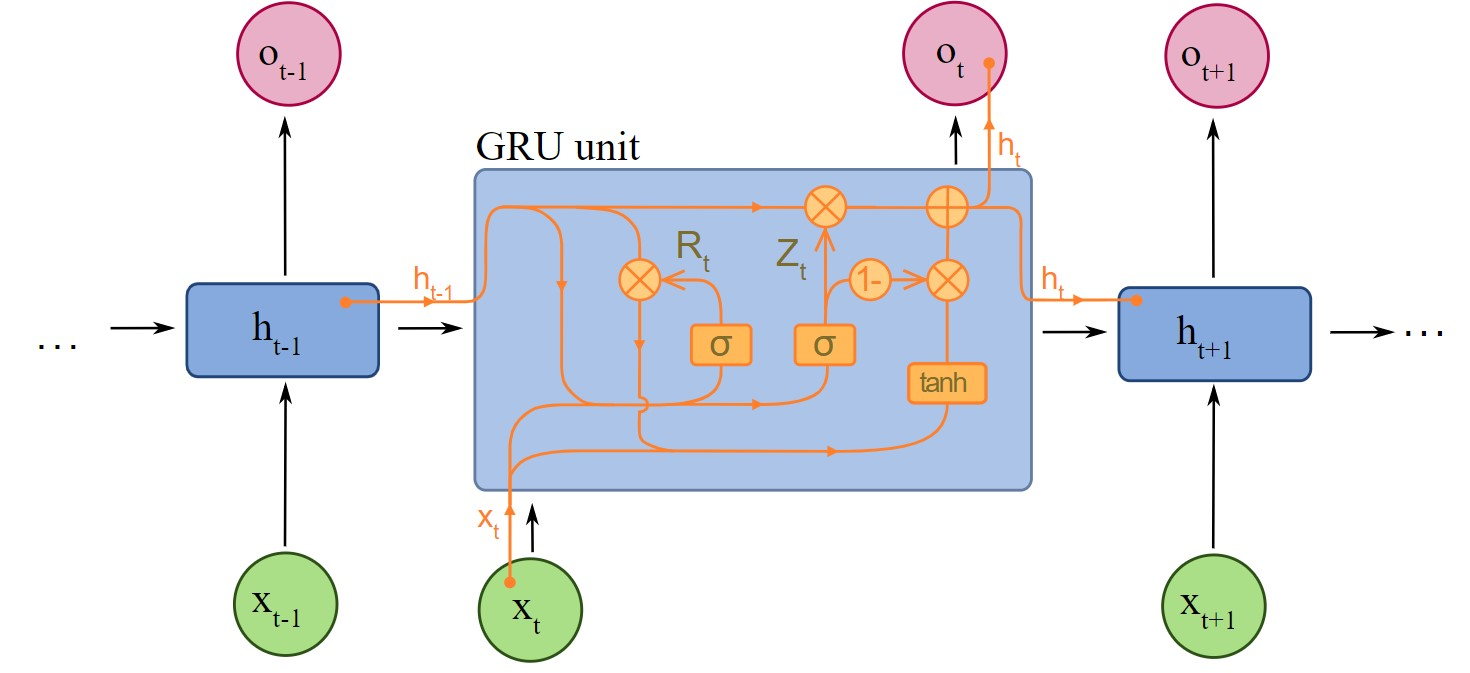
\includegraphics[width=.95\linewidth]{images/nn/layers/gru.jpg}
     \caption{GRU cell}
     \label{fig:gru}
   \end{minipage}
\end{figure}


\subsection{Transformers}

% ----------------------------------------------------------------------------------------------------
% Related work
% ----------------------------------------------------------------------------------------------------

% Level 1: Representation
% Level 2: objective
% Level 3: architecture
% Level 4: strategie

\chapter{Related works}

I will expose in this chapter the work that has already been done about music generation with deep neural networks.
In a first time, I will expose the different objectives of some implementations.
Then I will introduce 

% -------------------- Objectives  --------------------

\section{Objectives}        % Change the name

In this section, I will describe some examples of what it is possible to do with neural networks to generate music

\subsection{Generator}

First it is possible to create a music melody. It can be either monophonic (only one note played at one time) or polyphonic (several notes can be played at the same time).

It is also possible to create several musical parts at the same time. Each of them can be either monophonic or polyphonic.
The musical parts can be considered as different instruments or voices for a Chorale.
The challenge is to create musical parts that work together.

\subsection{Accompaniment}

Given a melody, or some musical parts, the goal is to create new musical parts which can be combined with the input and be played together.

% -------------------- Music Representation--------------------

\section{Music Representation}

In this section, I will present different types of inputs the recent works are using.

\subsection{Audio Signal} 

The first of data used to create music is the audio signal. Some works \cite{oord_wavenet:_2016} have been done to generate some an music audio signal.
This signal can be represented either by its waveform \cite{oord_wavenet:_2016}, its Fourier Transform, or its spectrogram (figures \ref{fig:waveform_example}, \ref{fig:spectrogram_example}).

\begin{figure}[H]
   \begin{minipage}{0.5\textwidth}
     \centering
     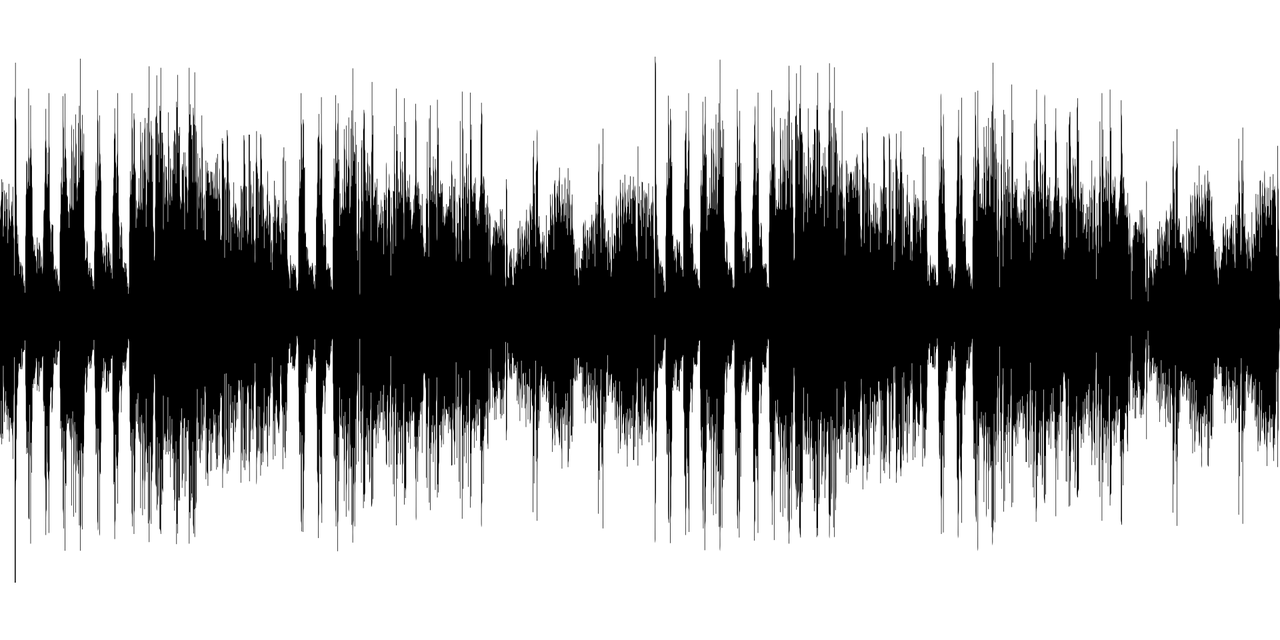
\includegraphics[width=.9\linewidth]{images/music/waveform/waveform.png}
     \caption{Example of an audio waveform}
     \label{fig:waveform_example}
   \end{minipage}\hfill
   \begin{minipage}{0.5\textwidth}
     \centering
     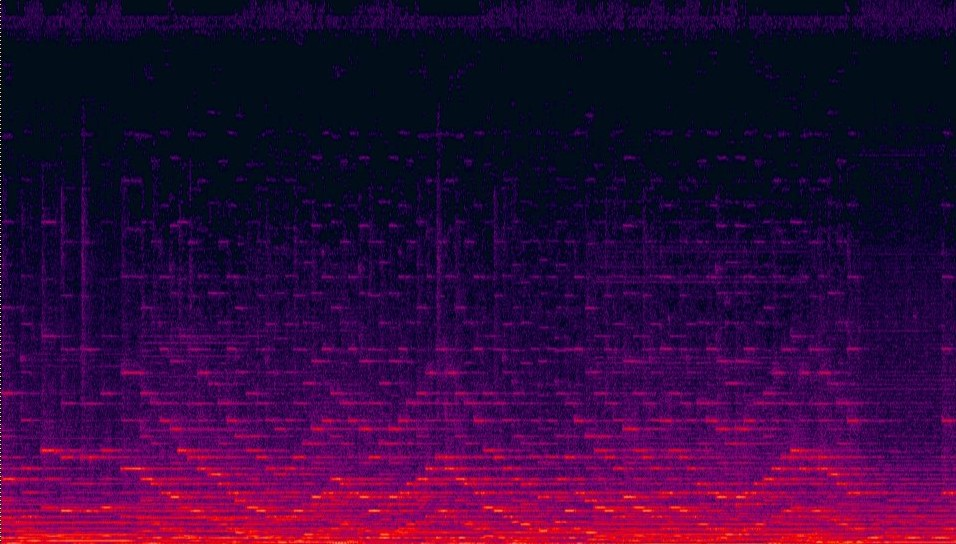
\includegraphics[width=\linewidth]{images/music/spectrogram/spectrogram.jpg}
     \caption{Example of audio spectrogram}
     \label{fig:spectrogram_example}
   \end{minipage}
\end{figure}

Using the audio signal allows the model to handle every aspect of the song at the same time, and every song in the same way.
The biggest issue of this method is that the number of points in time is incredibly huge. The usual sampling frequency is $48kHz$. 
Therefore, the challenge is to stay consistent through time.

\subsection{MIDI Signal}

Most of the work done on music generation is using the \textit{MIDI} representation (or any other translation of midi like pianoroll or text).

\subsubsection{Pianoroll}

The pianoroll representation can be considerate as an image so usual deep learning methods on images can  be applied \cite{huang_counterpoint_2017}.

\begin{figure}[H]
   \begin{minipage}{0.5\textwidth}
     \centering
     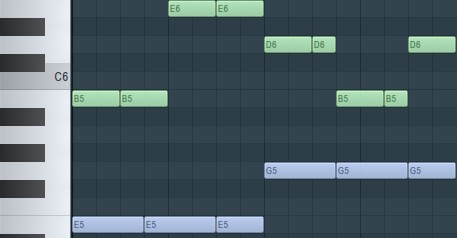
\includegraphics[width=.9\linewidth]{images/music/pianoroll/pianoroll_small.jpg}
   \end{minipage}\hfill
   \begin{minipage}{0.5\textwidth}
     \centering
     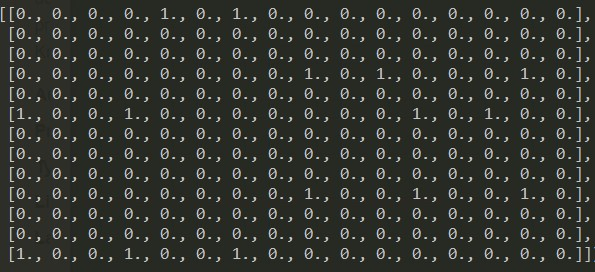
\includegraphics[width=\linewidth]{images/music/pianoroll/pianoroll_small_array.jpg}
   \end{minipage}
 \caption{Example of correspondence between a pianoroll representation and an array}
 \label{fig:pianoroll_to_array}
\end{figure}

The figure \ref{fig:pianoroll_to_array} shows a very naive example of how to convert a pianoroll view to an array.

\subsubsection{Text}

Another approach is to convert the MIDI format into text. \cite{hadjeres_deepbach:_2016}

\begin{figure}[H]
   \begin{minipage}{0.5\textwidth}
     \centering
     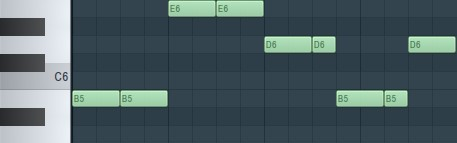
\includegraphics[width=.9\linewidth]{images/music/pianoroll/pianoroll_small_2.jpg}
   \end{minipage}\hfill
   \begin{minipage}{0.5\textwidth}
     \centering
     B5, \_, B5, \_, E6, \_, E6, \_, D6, \_, D6, B5, \_, B5, D6, \_ 
   \end{minipage}
 \caption{Example of correspondence between a pianoroll representation and a text}
 \label{fig:pianoroll_to_text}
\end{figure}

The figure \ref{fig:pianoroll_to_text} shows as simple example of how it is possible to convert an pianoroll view to a text.

However, using text to represent image usually force the framework to work only in a monophonic way.

% TODO: Speak about Word2Vec


\subsubsection{Chords}

This is the last approach I will describe in this paper.
As the same way as Jazz music, it is possible to simplify the description of a musical piece by writing down the chords.

\begin{figure}[H]
   \begin{minipage}{0.5\textwidth}
     \centering
     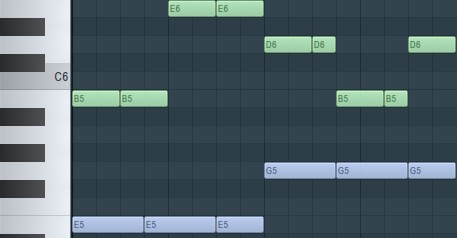
\includegraphics[width=.9\linewidth]{images/music/pianoroll/pianoroll_small.jpg}
   \end{minipage}\hfill
   \begin{minipage}{0.5\textwidth}
     \centering
     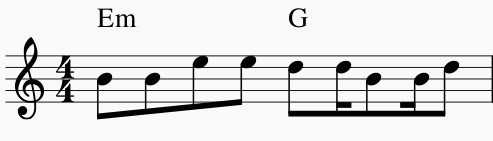
\includegraphics[width=.9\linewidth]{images/music/stave/stave_with_chords.jpg}
   \end{minipage}
 \caption{Example of correspondence between a pianoroll and its chords representation}
 \label{fig:pianoroll_to_chords}
\end{figure}

For instance, in the figure \ref{fig:pianoroll_to_chords}, the bass line can be simplified by considering the chords.
The chords are then writen and be considered as notes.


% TODO: Speak about BachBot
%       Survey descritpion 
% Note that a somehow similar model has been used for polyphonic music generation in
% the BachBot system [66] (analyzed in Section 7.3.1.3). In this model, for each time step, the
% various notes are represented as a sequence and a special delimiter symbol (|||) indicates
% the next time frame (with constant time step of an eighth note __(
% ). Notes are ordered, in a
% descending pitch (soprano voice being the first one). Each note is encoded as its MIDI pitch
% value and a boolean indicating if it is tied to a note at the same pitch from previous frame.
% An example is shown at Figure 4.8, encoding two successive chords (the first having the


% TODO: Speak about Chords2Vec
%       Survey descritpion 
% Note that a somehow similar model has been used for polyphonic music generation in
% the BachBot system [66] (analyzed in Section 7.3.1.3). In this model, for each time step, the
% various notes are represented as a sequence and a special delimiter symbol (|||) indicates
% the next time frame (with constant time step of an eighth note (<croche symbol>). Notes are ordered, in a
% descending pitch (soprano voice being the first one). Each note is encoded as its MIDI pitch
% value and a boolean indicating if it is tied to a note at the same pitch from previous frame.
% An example is shown at Figure 4.8, encoding two successive chords (the first having the
% duration of a quarter note) and the second one possessing a fermata (noted as (.)).


% -------------------- Encoding --------------------

\section{Encoding}

\subsection{Features}

It is possible to extract features from the data to help the neural network to understand how music works.
\begin{itemize}
    \item The first option is to do it manually and give the features as an input of the model
    \item The second option is to let the model learn it by itself. This is the choice I have made for this project.
\end{itemize}

\subsubsection{Metadata}

The features that can be passed as an input to the model can also be metadata as the time signature or the key of the music...
In this project I chose to not include any metadata in the model because of the difficulty to find or reconstruct them for the available dataset.

\subsection{Tensor encoding}

It is possible to extract two different methods on how to encode the tensor which will be given to the neural network

The first method is the \textit{value encoding}.
It is means that the values in the input and/or output tensor are actually meaning full.
For example, it can be an integer which is the pitch of a note.

The second method is called \textit{item encoding}.
Instead of having the number of the pitch in the tensor (let's say $60$), it will be a very sparse tensor with a bunch on $0$ and a $1$ at the position $60$ in the pitch dimension.
This values stored in the tensors can be considered as \textit{activation} values.
This is the retained method in this work.


\section{Architectures}

In this section, I will present different architectures that have already been used for music generation. It will expose the architecture of my project in the section \ref{sec:model_architecture}.

\subsection{RBM}

\subsection{AE}

\subsection{VAE}

\subsection{GAN}

\subsection{Reinforcement learning}

\section{Generation Process}

\subsection{Sampling}

\subsection{Input Manipulation}

\subsection{Feed forward and RNN architecture}

% ----------------------------------------------------------------------------------------------------
% Contribution
% ----------------------------------------------------------------------------------------------------
\newpage
\chapter{Contribution}
\label{chap:contribution}

\section{Objectives}

As a musician, I wanted to create an model architecture who could copy the way I think about music.
The challenge is to use only one trained model to be able to 
\begin{itemize}
    \item Generate music with several musical parts (meaning several instruments)
    \item Create a accompaniment from a melody
    \item Create a melody from a accompaniment
    \item Create a music part from other musical parts
\end{itemize}
The created model can also handle missing data (for example a missing measure from a instrument).

To summarize, the objective is to create a unique trained model which can generate or arrange a musical piece whatever is already present or missing.

\section{Data representation}

This project works with MIDI data. These music representation is explained in the section \ref{seq:midi}. \\
The shortest beat division is a quarter of a beat (sixteenth note: \musSixteenth) \\
The considered music are binary and with 4 beats per measure. \\
Because I think that a measure can be consider as an entire object (with its rhythm, its chords ...), I chose to divide music by measure. Thus, a time step for the neural network is the representation of an entire measure.
The shape of shape of a tensor representing a measure will be \texttt{(16, 128, channels)}:
\begin{itemize}
    \item \texttt{16} is the number of sixteenth notes (\musSixteenth) is a measure.
    \item \texttt{128} is the number of different MIDI notes possible (from $0$ to $127$).
    \item \texttt{channels} $\in \{1, 2\}$ is explained in the sections \ref{seq:poly} and \ref{seq:mono}.
\end{itemize}

The number of instruments is fixed and are different inputs of the neural network.
Hence, for one instrument, its associated tensor has a shape of \texttt{(nb\_measures, 16, 128, channels)}. \texttt{nb\_measures} is the number of measures considered.

\subsection{Polyphonic music}
\label{seq:poly}

For polyphonic music, the number of \texttt{channels} it $2$.

The first channel is called the \textit{activation} channel. The value is either $1$ for a played note or $0$ for a non-played note.

The second channel is called the \textit{duration} channel. The value is an integer corresponding of \textit{"how many sixteenth notes (\musSixteenth) it lasts"}.
The table \ref{tab:duration} shows the correspondence between the value of the duration channel and the musical length representation.

\begin{table} [ht]
    \begin{center}
        \begin{tabular} {c|c}
            Duration value & Musical length \\
            \hline
            $1$ & \musSixteenth \\
            $2$ & \musEighth \\
            $3$ & \musEighthDotted \\
            $4$ & \musQuarter \\
            $5$ & $\musQuarter_{\smile}$\musSixteenth \\
            $6$ & \musQuarterDotted \\
            $7$ & $\musQuarter_{\smile} \musEighthDotted$ \\
            $8$ & \musHalf \\
            $9$ & $\musHalf_{\smile} \musSixteenth$ \\
            $10$ & $\musHalf_{\smile} \musEighth$ \\
            $11$ & $\musHalf_{\smile} \musEighthDotted$ \\
            $12$ & \musHalfDotted \\
            $13$ & $\musHalfDotted_{\smile} \musSixteenth$ \\
            $14$ & $\musHalfDotted_{\smile} \musEighth$ \\
            $15$ & $\musHalfDotted_{\smile} \musEighthDotted$ \\
            $16$ & \musWhole \\
        \end{tabular}
        \caption{Correspondence between duration value and musical length}
        \label{tab:duration}
    \end{center}
\end{table}

If a note is note activated (activation channel $ = 0$), then the duration channel is set to $0$ too.

\begin{equation}
    \texttt{channel}_{\texttt{activation}} = 0 \iff \texttt{channel}_{\texttt{duration}} = 0
\end{equation}

\subsection{Monophonic Music}
\label{seq:mono}

The goal was too reduce the memory space a simplify the model for monophonic music.
Since monophonic music can means there is a maximum of one note played simultaneously at a time $t$, I chose to not consider the rests and consider that every notes last until an another note is played.\\
Thus, I get read of duration channel and the number of \texttt{channels} $ = 1$.

An \textit{additional note} is inserted which is the $note_{continue}$.
The tensor shape of a step is now \texttt{(16, 128 + 1, 1)}.
When $note_{continue}$ is set to $1$, it means there is no new note to be played.
And when $note_{continue}$ is set to $0$, it means a new notes has to be played.

\begin{equation}
    note_{continue} = 1 \implies \forall note \in notes_{[0:128]}, note = 0
\end{equation}

\begin{equation}
    note_{continue} = 0 \implies \exists note \in notes_{[0:128]}, note = 1
\end{equation}

And since I consider in this part only monophonic music, there is only on note (included $note_{continue}$ per each time division)

\begin{equation}
    \exists! note \in notes_{[0:129]}, note = 1
\end{equation}




\section{Model Architecture}
\label{sec:model_architecture}
Section text

% ----------------------------------------------------------------------------------------------------
% Experiments
% ----------------------------------------------------------------------------------------------------
\chapter{Experiments}

% ----------------------------------------------------------------------------------------------------
% Conclusion
% ----------------------------------------------------------------------------------------------------

\chapter{Conclusion}
My Conclusion

% ----------------------------------------------------------------------------------------------------
% Future work
% ----------------------------------------------------------------------------------------------------

\section*{Future work}
Future work
\newpage

% ####################################################################################################
% ####################################################################################################
% Bibliography
% ####################################################################################################
% ####################################################################################################
\bibliographystyle{plain}
\bibliography{biblio/Dissertation.bib}
% \printbibliography

% ####################################################################################################
% ####################################################################################################
% Appendix
% ####################################################################################################
% ####################################################################################################

\appendix

% \chapter{Full experimental results}

\end{document}

% Photographs, Illustrations and Other Attachments
% [For soft-bound, paper copy for Examination/Re-examination] Photographic and other illustrations that are to be included in the bound copy of the thesis have to be securely mounted using double-faced tape. Photograph album pockets or slits in the page are not adequate. In no circumstances should ‘cellophane tape’ or a similar material be used for any purpose in a copy of the thesis. All copies of the thesis should contain original photographs. Subsidiary papers and other loose material should be bound in wherever possible. If this is not possible, an adequately guarded pocket for each material should be provided at the end of the thesis. Any such loose material (and corrigenda sheets, if not bound in) should bear the candidate’s name, initials and degree.
% Photographic and other illustrations (e.g. line drawings, maps, musical scores, etc.) which need to be uploaded in the ETD system should be inserted in the thesis in PDF format as far as possible.
